% -*- latex -*-
%%%%%%%%%%%%%%%%%%%%%%%%%%%%%%%%%%%%%%%%%%%%%%%%%%%%%%%%%%%%%%%%
%%%%%%%%%%%%%%%%%%%%%%%%%%%%%%%%%%%%%%%%%%%%%%%%%%%%%%%%%%%%%%%%
%%%%
%%%% This text file is part of the source of 
%%%% `Parallel Programming in MPI and OpenMP'
%%%% by Victor Eijkhout, copyright 2012-2020
%%%%
%%%% mpi-performcollective.tex : performance issues
%%%%
%%%%%%%%%%%%%%%%%%%%%%%%%%%%%%%%%%%%%%%%%%%%%%%%%%%%%%%%%%%%%%%%
%%%%%%%%%%%%%%%%%%%%%%%%%%%%%%%%%%%%%%%%%%%%%%%%%%%%%%%%%%%%%%%%

\Level 0 {Performance considerations}

In this section we will consider how collectives can be implemented in
multiple ways, and the performance implications of such decisions.
You can test the algorithms described here using \indexterm{SimGrid}
(section~\ref{tut:simgrid}).

\Level 1 {Scalability}

We are motivated to write parallel software from two considerations.
First of all, if we have a certain problem to solve which normally
takes time~$T$, then we hope that with $p$ processors it will take time~$T/p$.
If this is true, we call our parallelization scheme \indextermbus{scalable}{in time}.
In practice, we often accept small extra terms:
as you will see below, parallelization often adds a term $\log_2p$
to the running time.

\begin{exercise}
  Discuss scalability of the following algorithms:
  \begin{itemize}
  \item
    You have an array of floating point numbers.
    You need to compute the sine of each
  \item You a two-dimensional array, denoting the interval~$[-2,2]^2$.
    You want to make a picture of the \indexterm{Mandelbrot set},
    so you need to compute the color of each point.
  \item The primality test of exercise~\ref{ex:primetest}.
  \end{itemize}
\end{exercise}

There is also the notion that a parallel algorithm can be
\indextermbus{scalable}{in space}: more processors gives you more memory
so that you can run a larger problem.

\begin{exercise}
  Discuss space scalability in the context of modern processor design.
\end{exercise}

\Level 1 {Complexity and scalability of collectives}

\Level 2 {Broadcast}

\heading{Naive broadcast}

Write a broadcast operation where the root does an \indexmpishow{MPI_Send} to
each other process.

What is the expected performance of this in terms of $\alpha,\beta$?

Run some tests and confirm.

\heading{Simple ring}

Let the root only send to the next process, and that one send to its
neighbour. This scheme is known as a \indexterm{bucket brigade}; see
also section~\ref{sec:bucketbrigade}.

What is the expected performance of this in terms of $\alpha,\beta$?

Run some tests and confirm.

\begin{figure}[ht]
  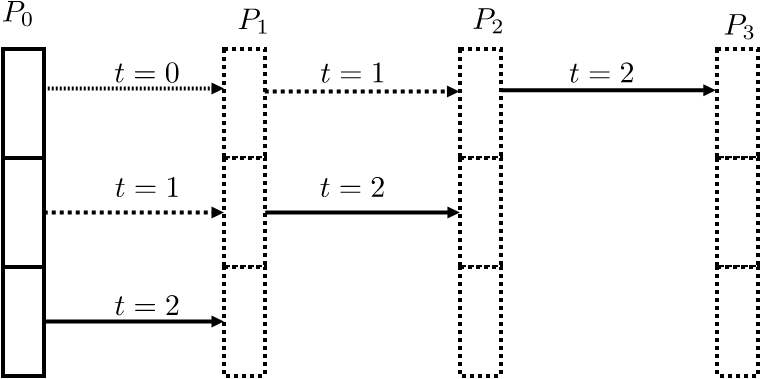
\includegraphics[scale=.6]{bucketpipe}
  \caption{A pipelined bucket brigade}
  \label{fig:pipe-bucket}
\end{figure}

\heading{Pipelined ring}

In a ring broadcast, each process needs to receive the whole message
before it can pass it on. We can increase the efficiency by breaking
up the message and sending it in multiple parts.
(See figure~\ref{fig:pipe-bucket}.)
This will be
advantageous for messages that are long enough that the bandwidth cost
dominates the latency.

Assume a send buffer of length more than~1. Divide the send buffer
into a number of chunks. The root sends the chunks successively to the
next process, and each process sends on whatever chunks it receives.

What is the expected performance of this in terms of $\alpha,\beta$?
Why is this better than the simple ring?

Run some tests and confirm.

\heading{Recursive doubling}

Collectives such as broadcast can be
\emph{implemented}
through
\index{doubling!recursive|see{recursive doubling}}%
\indexterm{recursive doubling},
where the root sends to another process, then the root and the other
process send to two more, those four send to four more, et cetera.
However, in an actual physical architecture this scheme can be
realized in multiple ways that have drastically different performance.

First consider the implementation where process~0 is the root, and it
starts by sending to process~1; then they send to 2 and~3; these four
send to~4--7, et cetera. If the architecture is a linear array of
procesors, this will lead to \indexterm{contention}: multiple messages
wanting to go through the same wire. (This is also related to the
concept of \indextermsub{bisecection}{bandwidth}.)

In the following analyses we will assume \indexterm{wormhole routing}:
a~message sets up a path through the network, reserving the necessary
wires, and performing a send in time independent of the distance
through the network. That is, the send time for any message can be
modeled as \[ T(n)=\alpha+\beta n \] regardless source and
destination, as long as the necessary connections are available. 

\begin{exercise}
  \label{ex:bcast-doubling-block}
  Analyze the running time of a recursive doubling broad cast as just
  described, with wormhole routing.

  Implement this broadcast in terms of blocking MPI send and receive calls.
  If you have SimGrid available, run
  tests with a number of parameters.
\end{exercise}

The alternative, that avoids contention, is to let each doubling stage
divide the network into separate halves. That is, process~0 sends
to~$P/2$, after which these two repeat the algorithm in the two halves
of the network, sending to $P/4$ and $3P/4$ respectively.

\begin{exercise}
  Analyze this variant of recursive doubling. Code it and measure
  runtimes on SimGrid.
\end{exercise}

\begin{exercise}
  \label{ex:bcast-doubling-nonblock}
  Revisit exercise \ref{ex:bcast-doubling-block} and replace the
  blocking calls by nonblocking \indexmpishow{MPI_Isend}~/ \indexmpishow{MPI_Irecv} calls.

  Make sure to test that the data is correctly propagated.
\end{exercise}

MPI implementations often have multiple algorithms, which they
dynamicaly switch between. Sometimes you can determine the choice yourself
through environment variables.

\begin{taccnote}
  For \indextermbus{Intel}{MPI}, see
  \url{https://software.intel.com/en-us/mpi-developer-reference-linux-i-mpi-adjust-family-environment-variables}.
\end{taccnote}
